\documentclass[11pt]{article}
\usepackage[margin=2.2cm]{geometry}
\usepackage{amsmath,amssymb}
\usepackage{graphicx}
\usepackage{booktabs}
\usepackage{xcolor}
\usepackage{siunitx}
\usepackage[colorlinks=true,linkcolor=blue,urlcolor=blue]{hyperref}
\usepackage{parskip}

\newcommand{\rC}{r_C}
\title{\vspace{-1.2cm}\textbf{SINDy on the Four Moreton-Bay Tide Gauges}\\[2pt]
\large A side exercise: discovering a forced linear model from gauge data}
\author{PINN course --- Unit~1 data, Unit~3 (SINDy) method}
\date{\today}

\begin{document}
\maketitle
\vspace{-0.6cm}

\section*{The key idea}

\textbf{SINDy} (Sparse Identification of Nonlinear Dynamics) takes a measured
trajectory $\mathbf{x}(t)\in\mathbb{R}^n$, estimates its time derivative
$\dot{\mathbf{x}}(t)$, and looks for the \emph{sparsest} combination of candidate
functions that reproduces it:
\[
  \dot{\mathbf{x}} \;=\; \Theta(\mathbf{x})\,\Xi,
  \qquad
  \Theta(\mathbf{x}) = \big[\,1\;\;\mathbf{x}\;\;\mathbf{x}^{\otimes 2}\;\;\cdots\,\big],
\]
where each column of $\Theta$ is a candidate term and the columns of $\Xi$ are
made sparse by a thresholded least squares (STLSQ). The premise is that the
\emph{right} variables obey a \emph{closed, autonomous} law with only a few active
terms.

Here we test that premise on real course data: the \textbf{four tide gauges} of
Unit~1. The state is
$\mathbf{x}(t)=\big(\eta_{G1},\eta_{G2},\eta_{G3},\eta_{G4}\big)$, the noise-free
(\texttt{gauges\_clean}) water-level anomalies, sampled at $\Delta t=\SI{12}{s}$
over $\SI{10}{h}$ ($N=3001$ points). The twist: the bay is a \emph{linearised
shallow-water system}, and it is \textbf{forced} by an external river surge
$\psi(t)$ at the Brisbane River mouth --- a pulse peaking at $\psi\approx0.45$
around $t\approx\SI{2}{h}$, then decaying. So the honest model class is a
\emph{forced linear} system,
\[
  \boxed{\;\dot{\mathbf{x}} \;=\; A\,\mathbf{x} \;+\; \mathbf{b}\,\psi(t)\;}
\]
and the central question becomes: \emph{can SINDy see the forcing?}

\section*{What we ran}

Two fits, both with a constant\,$+$\,linear library and column-normalised STLSQ
(relative threshold $\lambda=0.05$); derivatives by central differences:
\begin{itemize}\itemsep1pt
  \item \textbf{(A) Autonomous} --- library $[\,1,\,\eta_{G1\ldots G4}\,]$ only:
        $\dot{\mathbf{x}}=A\mathbf{x}$.
  \item \textbf{(B) Controlled (SINDYc)} --- append the known forcing $\psi(t)$ as
        an extra column: $\dot{\mathbf{x}}=A\mathbf{x}+\mathbf{b}\,\psi$.
\end{itemize}
Each identified model is then integrated forward (RK4) from rest,
$\mathbf{x}(0)=\mathbf{0}$, and compared to the gauge data.

\section*{The discovered system}

The controlled fit returns a \emph{stable, oscillatory} forced linear model
(all entries $\times10^{4}$ for readability):
\[
  10^{4}A \;=\;
  \begin{pmatrix}
    +4.20 & +4.29 & -8.13 & -1.08\\
    +3.28 & +3.08 & -6.79 & -0.32\\
    +5.76 & +4.55 & -9.42 & -1.08\\
    +3.51 & -4.97 & +2.53 & -0.03
  \end{pmatrix},
  \qquad
  10^{4}\mathbf{b} \;=\;
  \begin{pmatrix} +0.31\\ +0.32\\ -0.02\\ +0.14 \end{pmatrix}.
\]

\textbf{Eigen-analysis of $A$.} Two lightly-damped oscillatory pairs,
\[
  \lambda \approx (-5.4\pm 9.0\,i)\times10^{-5}
  \;\;\text{and}\;\;
  (-5.4\pm 32\,i)\times10^{-5}\ \si{s^{-1}},
\]
i.e.\ resonant \textbf{periods $\approx\SI{19.3}{h}$ and $\approx\SI{5.4}{h}$},
each with an $e$-folding decay of $\approx\SI{5}{h}$. SINDy recovered the bay's
physical mode structure from four scalar timeseries, and $\max\mathrm{Re}(\lambda)
=-5.4\times10^{-5}<0$, so the model is stable to integrate forward.

\textbf{Forcing vector $\mathbf{b}$.} The surge enters predominantly through
$G1$ and $G2$ --- the gauges nearest (and across from) the river mouth --- and
$\approx 0$ at $G3$ (Tangalooma, in the Moreton-Island lee). The identified
forcing direction is physically where you would expect it.

\begin{figure}[h]
  \centering
  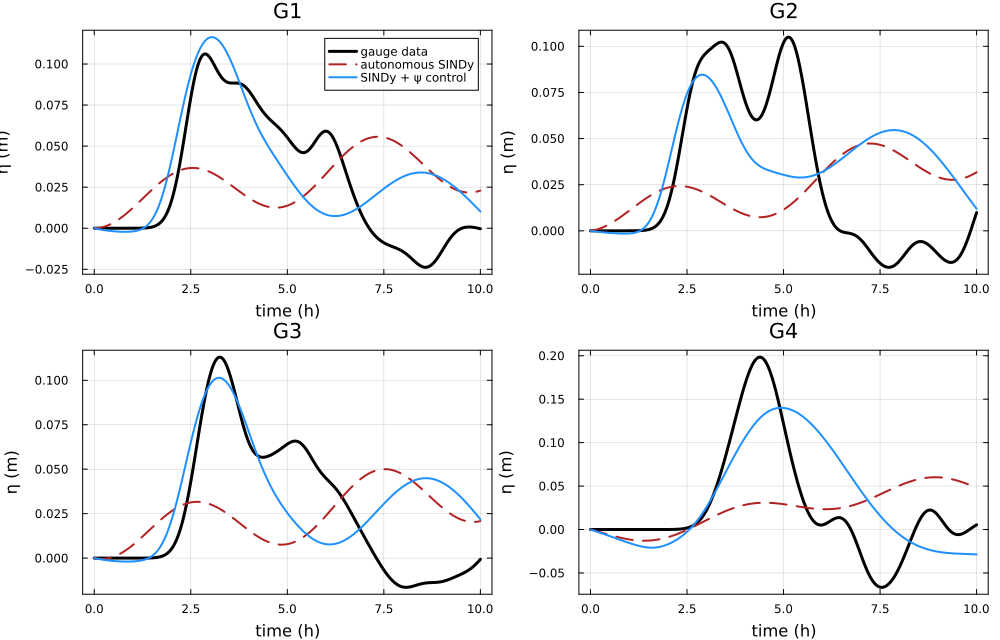
\includegraphics[width=\linewidth]{sindy_gauges.png}
  \caption{Each panel: gauge data (\textbf{black}) vs.\ the two identified models,
  integrated from rest. \textcolor{red}{\textbf{Autonomous SINDy}} (red dashed)
  has no forcing term, so from rest it never leaves rest --- it cannot manufacture
  the surge. \textcolor{blue}{\textbf{SINDy\,$+\,\psi$ control}} (blue) captures the
  onset, timing and primary peak of the surge response (near-exact at $G3$),
  driven by the recovered $\mathbf{b}\,\psi(t)$. It misses the secondary peaks and
  late ringing --- see the closure caveat below.}
\end{figure}

\section*{Three lessons}

\begin{enumerate}\itemsep2pt
  \item \textbf{Forced systems need a control input.} Autonomous SINDy fails
        outright: per-gauge reconstruction error $\approx 90$--$\SI{100}{\percent}$.
        With no forcing term, a model started from rest stays at rest. Adding the
        known $\psi(t)$ (SINDYc) is what makes the surge appear --- error drops to
        $\approx 57$--$\SI{80}{\percent}$ and the primary event is captured.
  \item \textbf{SINDy can recover real physical structure.} The eigenvalues of the
        identified $A$ are the bay's damped resonant modes ($\approx\SI{5.4}{h}$,
        $\approx\SI{19.3}{h}$), and $\mathbf{b}$ localises the forcing to the
        river-side gauges --- both physically meaningful, read straight off the
        coefficients.
  \item \textbf{Closure matters --- and four point-gauges are \emph{not} closed.}
        The residual misfit (secondary peaks, late ringing) is not a tuning
        failure: the gauges are a \emph{partial observation of a PDE field}, so the
        true gauge dynamics depend on the whole hidden bay state, and no
        four-state ODE can be exact. Closing the gap is the natural next step ---
        \textbf{time-delay embeddings} (HAVOK) or more observables.
\end{enumerate}

\section*{Why this is a good Unit-3 example}

It teaches SINDy's two central caveats at once on a real, multivariate,
\emph{forced} dataset --- (i) autonomous vs.\ control inputs, and (ii) the need for
a closed state --- and it threads Unit~3 back to the Unit~1 surge inverse problem,
where recovering exactly this $\psi(t)$ is the headline task.

\vspace{0.4cm}
\footnotesize\noindent\textbf{Data:} \texttt{units/unit\_01/data/\{gauges\_clean,
psi\_truth\}.csv}. \quad\textbf{Method:} central-difference $\dot{\mathbf{x}}$,
constant\,$+$\,linear library, column-normalised STLSQ. \quad Exploratory;
\texttt{sindy-explore} branch only.

\end{document}
